% ----------------------------------------------------------------------------------------\
% ---------------------------------------------------------------------------------------\
% --------------------------------------------------------------------------------------\
\section{Instrucciones}
% ----------------------------------------------------------------------------------------\
% ---------------------------------------------------------------------------------------\
% --------------------------------------------------------------------------------------\

\begin{enumerate}
    \item Implementación básica del Juego de la Vida
    \item Introducción a los Algoritmos Genéticos
    \item Implementación de Algoritmos Genéticos en el Juego de la Vida
\end{enumerate}

% ----------------------------------------------------------------------------------------\
% ---------------------------------------------------------------------------------------\
% --------------------------------------------------------------------------------------\
\section{Investigación}
% ----------------------------------------------------------------------------------------\
% ---------------------------------------------------------------------------------------\
% --------------------------------------------------------------------------------------\

\subsubsection*{¿Qué es el algoritmo Genético?}

Un algoritmo genético \texttt{(AG)} entonces es: una técnica de resolución de problemas 
que utiliza principios inspirados en la selección natural para solucionar problemas de 
optimización. La selección natural (evolución) como estrategia implica la creación, 
reproducción y adaptación de una población de posibles soluciones en un rango de generaciones.\\ 

Este enfoque de población se basa en que cada individuo representa una posible solución 
al problema, y la evolución de estos comienza por, la \textbf{creación} de los individuos, 
la \textbf{reproducción} para después hacer la óptima \textbf{selección} de los padres en 
una nueva reproducción y \textbf{mutación}, finalmente comprobar o evaluar su \textbf{aptitud}\\ 


\subsubsection*{Pasos que sigue}

\begin{center}
    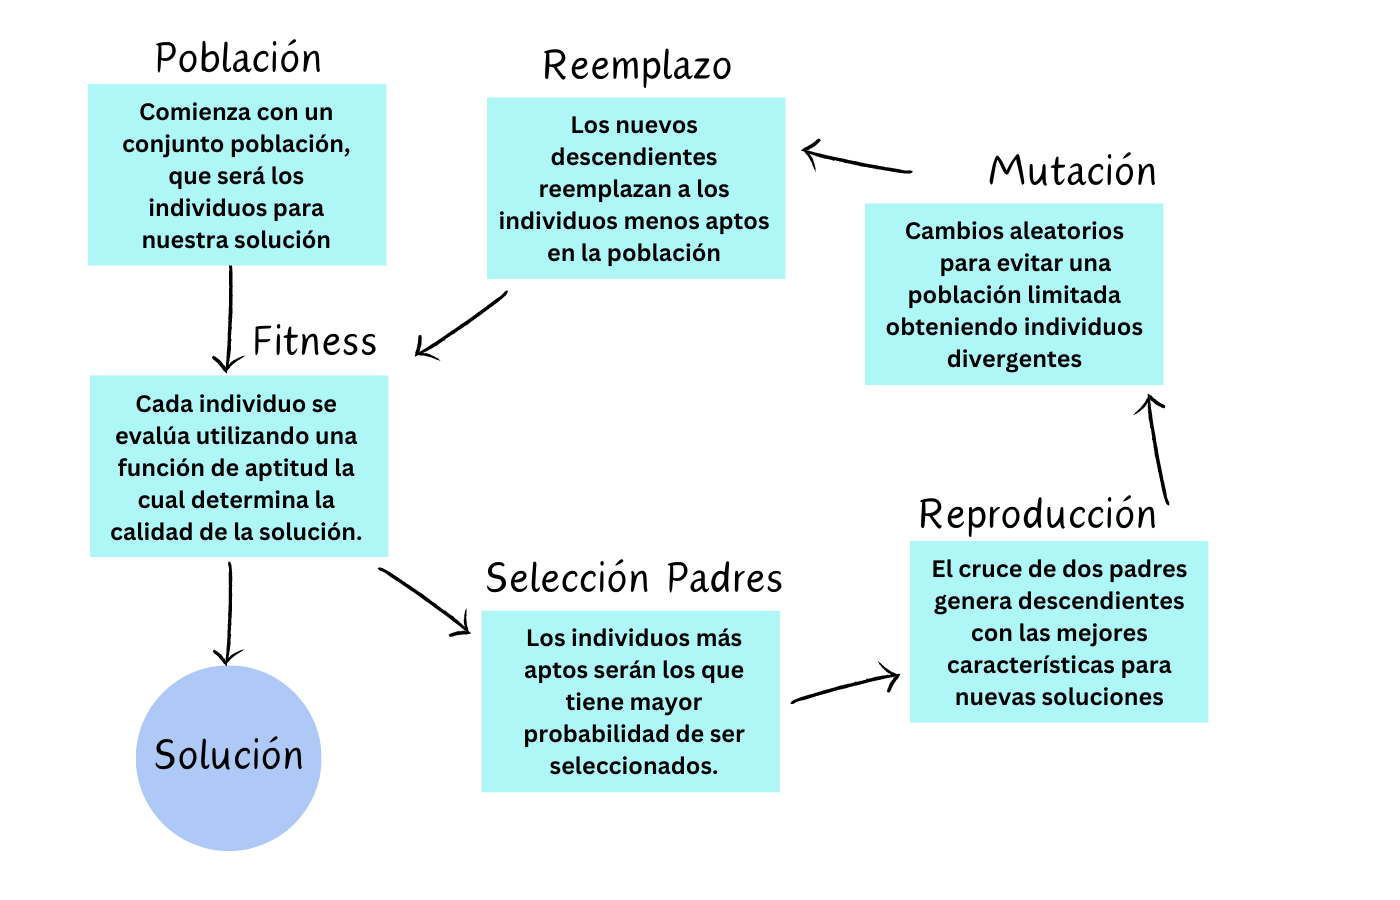
\includegraphics[scale = .4]{IMA/algo genetico.png}
\end{center}